\documentclass[tikz,border=10pt]{standalone}
\usepackage{tikz}
\usetikzlibrary{matrix}

\tikzset{
  cell/.style={draw=black!70, line width=1.0pt, minimum width=4.2cm, minimum height=1.05cm, align=center, text width=3.8cm, fill=none},
  head/.style={cell, draw=blue!70!black, line width=1.2pt},
  left/.style={cell, draw=green!50!black, line width=1.2pt}
}

\begin{document}
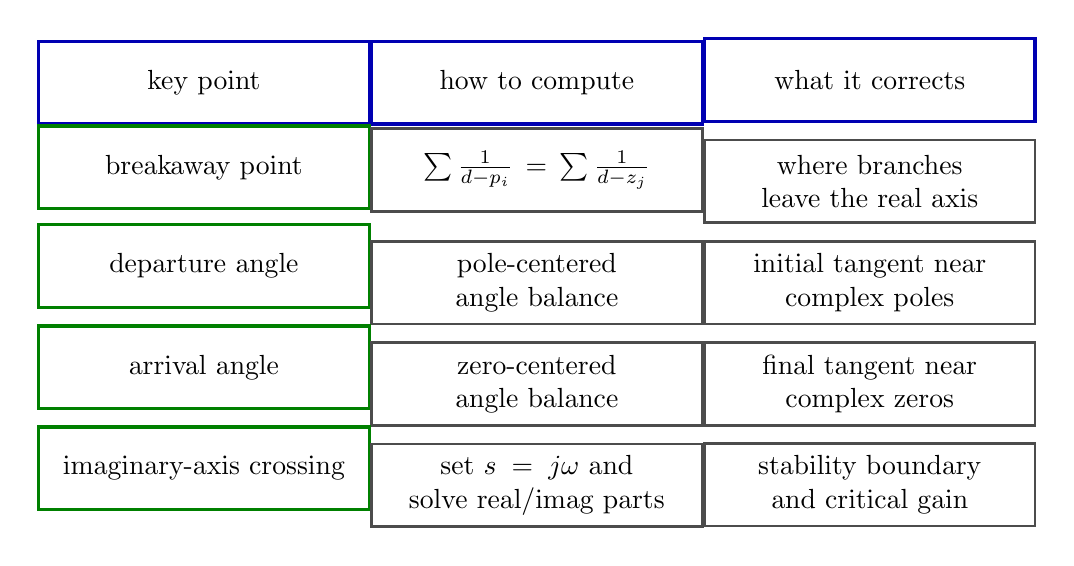
\begin{tikzpicture}
  \matrix[matrix of nodes, nodes in empty cells, row sep=-\pgflinewidth, column sep=-\pgflinewidth] {
    \node[head] {key point}; &
    \node[head] {how to compute}; &
    \node[head] {what it corrects}; \\
    \node[left] {breakaway point}; &
    \node[cell] {$\sum \frac{1}{d-p_i}=\sum \frac{1}{d-z_j}$}; &
    \node[cell] {where branches leave the real axis}; \\
    \node[left] {departure angle}; &
    \node[cell] {pole-centered angle balance}; &
    \node[cell] {initial tangent near complex poles}; \\
    \node[left] {arrival angle}; &
    \node[cell] {zero-centered angle balance}; &
    \node[cell] {final tangent near complex zeros}; \\
    \node[left] {imaginary-axis crossing}; &
    \node[cell] {set $s=j\omega$ and solve real/imag parts}; &
    \node[cell] {stability boundary and critical gain}; \\
  };
\end{tikzpicture}
\end{document}
